\documentclass[14pt]{beamer}
\usepackage[utf8]{inputenc}
\usepackage[english,russian]{babel}
\usepackage{graphicx}
\usetheme{Berlin}
\begin{document}
	\author{В.А. Преловский}
	\title{Контроль версий кода}
	%\subtitle{}
	%\logo{}
	%\institute{}
	%\date{}
	%\subject{}
	%\setbeamercovered{transparent}
	%\setbeamertemplate{navigation symbols}{}
	\frame[plain]{\maketitle}
	
	\begin{frame}
		\frametitle{Что такое контроль версий?}
		
		Система контроля версий (СКВ) - это система, регистрирующая изменения в одном или нескольких файлах с тем, чтобы в дальнейшем была возможность вернуться к определјнным старым версиям этих файлов.
		Мы чаще всего используем её для исходных кодов программ, но на самом деле под версионный контроль можно поместить файлы практически любого типа.
	\end{frame}

	\begin{frame}
		\frametitle{Основное практическое использование}
		
		{\small Такие системы наиболее широко используются при разработке программного обеспечения для хранения исходных кодов разрабатываемой
		программы. Однако они могут с успехом применяться и в других областях,
		в которых ведјтся работа с большим количеством непрерывно изменяющихся электронныхдокументов. В частности, системы управления версиями применяются в САПР, обычно в составе систем управления данными об
		изделии (PDM) . Управление версиями используется в инструментах конфигурационного управления (Software Configuration Management Tools).
	}
	\end{frame}

\begin{frame}
	\frametitle{Возможности систем контроля версий}
	{\footnotesize 
		\begin{itemize}
			\item Позволяют создавать разные варианты одного документа, т. н. ветки,
			с общей историей изменений до точки ветвления и с разными после
			неё.
			\item Дают возможность узнать, кто и когда добавил или изменил конкретный набор строк в файле.
			\item Ведут журнал изменений, в который пользователи могут записывать пояснения о том что и почему они изменили в данной версии.
			\item 	Контролируют права доступа пользователей, разрешая или запрещая	чтение или изменение данных, в зависимости от того, кто запрашивает это действие
		\end{itemize}
	}
\end{frame}

\begin{frame}
	\frametitle{Распределенные системы контроля версий}
	
{\scriptsize 	И в ситуации, когда главный сервер может "умереть в игру вступают распределјнные системы контроля версий (РСКВ) .
	В таких системах как Git Mercurial Bazaar или Darcs клиенты не просто выгружают последние версии файлов, а полностью копируют весь репозиторий. Поэтому в случае, когда "умирает" сервер, через который шла работа любой клиентский репозиторий может быть скопирован обратно на сервер, чтобы восстановить базу данных. Каждый раз, когда клиент забирает свежую версию файлов, он создајт себе полную копию всех данных (см. рисунок ниже) .
}
\end{frame}

\begin{frame}
	\frametitle{Распределенные системы контроля версий}
	\centering
	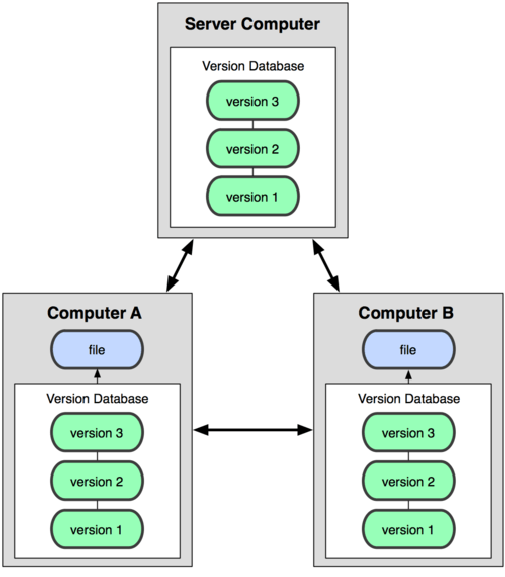
\includegraphics[width=0.5\textwidth]{DVCS}

\end{frame}

\begin{frame}
	\frametitle{Литература}
	\begin {thebibliography}{10}
	\bibitem {Wikiarticle}
	{\sc Статья в Википедии},{\href{https://ru.wikipedia.org/wiki/Система_управления_версиями}{о системах контроля версий кода}}
	
	\bibitem {OnlineBook}
	{\sc Книга Скотта Шакона},{\href{https://git-scm.com/book/en/v2}{Онлайн книга Скотта Шакона Pro Git}}
	\end {thebibliography}
\end{frame}

\end{document}